\maketitle
 
\begin{abstract}
{\itshape
\noindent % Better alignment for abstract in Garamond
% Optional: Use slightly smaller size for abstract
% \small
% Add subtle spacing
\setstretch{1.05}
\noindent
Starting from the operadic formalism of two-dimensional conformally invariant quantum field theory and its generalizations, as developed in the notion of a Chiral Algebra by Beilinson-Drinfeld \cite{BD}, we develop a comprehensive geometric framework for bar-cobar duality of chiral algebras via configuration space integrals and logarithmic differential forms. We construct an explicit geometric realization of the bar complex
for chiral algebras, establishing functoriality, uniqueness up to canonical isomorphism,  and essential surjectivity onto the category of conilpotent chiral coalgebras. The dual cobar construction for chiral coalgebras is in parallel realized through Čech-type complexes on configuration spaces. We demonstrate that the corresponding (co)differential given by residues along boundary divisors satisfies $d^2 = 0$, and realize Bar-Cobar duality as a direct manifestation of Poincare-Verdier duality over the global configuration space. 

\medskip
\noindent
The constructions naturally encode canonical $A_\infty$ structures, with higher homotopies determined by Arnold-Orlik-Solomon relations among logarithmic (distributional) forms on boundary strata. These geometric dualities vastly extend the notion of Koszul duality for chiral algebras to a more general theory of \textbf{Koszul dual pairs}, servicing a range of applications from deformation theory, bulk-boundary correspondences in supersymmetric gauge and field theory, to modern approaches to quantum gravity via twisted holography.

\medskip
\noindent
In service of these applications we treat Koszul duality computationally via the \textbf{The Prism Principle:} Just as a physical prism decomposes white light into its spectrum, our geometric bar complex acts as a mathematical prism for chiral algebras. The logarithmic forms $d\log(z_i - z_j)$ on configuration spaces $\overline{C}_n(X)$ separate the global chiral structure into its constituent OPE coefficients through residue calculus. Each collision divisor $D_{ij}$ corresponds to a specific "spectral line" --- an operator product channel --- with residues extracting the corresponding structure constants. This geometric spectroscopy provides both conceptual clarity and computational power, transforming abstract algebraic structures into concrete geometric data.
}
\end{abstract}
\tableofcontents

\section{Introduction}

% Optional: Drop cap for the first letter (elegant in Garamond)
% Requires lettrine package
% \usepackage{lettrine}
% \lettrine[lines=3,lraise=0.1,loversize=0.15]{C}{lassical} approaches...

\subsection{Context and Motivation}


\noindent\textbf{The Fundamental Question:} What is the correct homological algebra for chiral algebras? 
Classical approaches using Hochschild or cyclic homology fail to capture the intrinsic higher dimensional complexity. Following 
Grothendieck's principle that \textit{a mathematical object is determined by its category of representations}, 
we show the bar complex --- realized geometrically on configuration spaces --- provides the natural answer.

\medskip
\noindent\textbf{The Geometric Prism:} Consider how a prism reveals the hidden spectrum within composite light. 
Similarly, the geometric bar complex acts as a \textit{prism} for chiral algebras:

\begin{center}
\begin{tikzcd}[column sep=large, row sep=large]
\text{Chiral Algebra } \mathcal{A} \arrow[r, "{\text{Bar}}"] \arrow[dr, dashed, "{\text{hidden}}"] & 
\bar{B}^{\text{ch}}(\mathcal{A}) = \bigoplus_n \Omega^n(\overline{C}_{n+1}(X)) \\
& \text{Structure coefficients } \{C_{ijk}^{\ell}\} \arrow[u, hook, "{\text{residues}}"]
\end{tikzcd}
\end{center}

The logarithmic forms $\eta_{ij} = d\log(z_i - z_j)$ act as the ``diffracting medium,'' separating the 
global chiral structure into its local components:
\begin{itemize}
\item Each collision divisor $D_{ij}$ corresponds to a specific ``wavelength'' (OPE channel)
\item Residues extract the ``intensity'' at that wavelength (structure coefficient)
\item The total spectrum reconstructs the original algebra via cobar construction
\end{itemize}

This prism analogy is mathematically precise: just as Fourier analysis decomposes functions into frequencies, 
the geometric bar complex decomposes chiral algebras into their operadic components.

\subsection{From Abstract to Concrete: Why Configuration Spaces?}

\noindent\textbf{The Fundamental Bridge:} Given an operad $\mathcal{P}$ and an algebra $A$ over $\mathcal{P}$, 
the bar construction $B_{\mathcal{P}}(A)$ is defined abstractly as a cotriple resolution. But why should 
this abstract construction have a geometric realization on configuration spaces?

The answer, following Lurie \cite{HA}, Ayala-Francis \cite{AF}, and Gaitsgory-Francis, lies in understanding 
chiral algebras through the lens of \emph{factorization homology}. We present a conceptual roadmap:

\begin{enumerate}
\item \textbf{Operads as Configuration Categories} (Lurie): The chiral operad is not just an abstract 
operad but the operad of \emph{disks} in the Riemann surface $X$

\item \textbf{Factorization as Locality} (Ayala-Francis): Chiral algebras are precisely those algebras 
compatible with the factorization structure of configuration spaces

\item \textbf{Bar as Derived Mapping Space} (Gaitsgory): The bar complex computes 
$\text{RHom}_{\text{FactAlg}}(\mathbb{1}, \mathcal{A})$ where $\mathbb{1}$ is the vacuum factorization algebra

\item \textbf{Geometric Realization} (Kontsevich): Configuration space integrals provide the explicit model
\end{enumerate}

This work synthesizes three mathematical traditions: (1) Beilinson-Drinfeld's algebraic approach via 
$\mathcal{D}$-modules, (2) Kontsevich's geometric perspective using configuration space integrals, and 

\begin{remark}[Grothendieck's Perspective]
Following Grothendieck's principle that ``all dualities can be realized via Poincare-Verdier duality,'' our approach views chiral algebras not through their explicit presentations but through their bar complexes. The geometric realization on configuration spaces provides:
\begin{itemize}
\item \textbf{Functoriality:} Natural transformations = geometric correspondences
\item \textbf{Universality:} The bar construction is the ``free resolution'' in the chiral world
\item \textbf{Relative perspective:} Working over configuration spaces allows us to treat local and global geometry simultaneously
\item \textbf{Extending Koszul Duality:} By working with the more general Bar-Cobar duality realized as Poincare-Verdier duality of the configuration space, we can extend the notion of a Koszul dual pair to encompass more general dualities.
\end{itemize}
As we will see later, the shift in view from factorizable D-modules over local curves to coherent geometric systems living over configuration spaces brings us into contact with subjects ranging from topological string amplitudes and gromov-witten invariants to integrable systems.
\end{remark}

\subsection{Physical Motivation and Applications}

Our geometric bar-cobar duality has direct applications to:

\begin{enumerate}
\item \textbf{2d Conformal Field Theory:} The bar complex computes:
\begin{itemize}
\item Conformal blocks as cohomology classes
\item BRST cohomology of string worldsheets
\item Sewing/factorization properties via boundary stratification
\end{itemize}

\item \textbf{Holographic Duality:} Koszul dual pairs of chiral algebras correspond to:
\begin{itemize}
\item Bulk/boundary dualities in AdS$_3$/CFT$_2$
\item The geometric bar complex computes boundary observables
\item MC elements encode bulk gauge fields
\end{itemize}

\item \textbf{Quantum Groups:} At critical level $k = -h^\vee$:
\begin{itemize}
\item Chiral algebras become singular, requiring our extended framework
\item Bar complex resolves singularities via configuration spaces
\item Connects to center of quantum groups at roots of unity
\end{itemize}
\end{enumerate}

\begin{remark}[String Theory Connection]
In string theory, our construction appears as:
\begin{itemize}
\item Worldsheet CFT: Configuration spaces = moduli of punctured Riemann surfaces
\item Vertex operators: Chiral algebra elements = local operators in CFT
\item String amplitudes: Bar complex differential = BRST operator
\item The prism principle: Decomposition into color-ordered amplitudes
\end{itemize}
\end{remark}

\begin{tcolorbox}[title=Key Contributions of This Work]
\begin{enumerate}
\item \textbf{Geometric Realization:} First complete construction of bar complex for chiral algebras using configuration spaces and logarithmic forms

\item \textbf{Prism Principle:} Novel conceptual framework viewing the bar complex as decomposing chiral algebras into their spectral components

\item \textbf{Unification:} Bridges three perspectives:
   \begin{itemize}
   \item Beilinson-Drinfeld (algebraic)
   \item Kontsevich (geometric)
   \item Ayala-Francis (higher categorical)
   \end{itemize}

\item \textbf{Explicit Computations:} Concrete formulas for:
   \begin{itemize}
   \item Structure constants via residues
   \item Maurer-Cartan elements geometrically
   \item Koszul duality pairs
   \end{itemize}

\item \textbf{Extensions:} Framework handles:
   \begin{itemize}
   \item Curved/filtered algebras
   \item Critical level phenomena
   \item Holographic dualities
   \end{itemize}
\end{enumerate}
\end{tcolorbox}

(3) Ayala-Francis's higher categorical framework of factorization homology.
 
\subsection{Motivation from Physics and Mathematics}
 
In two-dimensional conformal field theory, local operators $\phi(z)$ depend holomorphically on positions and interact through operator product expansions (OPEs) when points collide. The mathematical formalization of this structure via chiral algebras, introduced by Beilinson and Drinfeld \cite{BD04}, encodes locality through sophisticated factorization structures on the Ran space of algebraic curves.
 
The homological algebra of such objects should naturally remember collision patterns and encode the geometry of how points come together. The physical intuition suggests that when operators collide, the singularities in their correlation functions should be captured by residues along collision divisors. Moreover, the associativity of the operator product should emerge from the consistency of different orders of collision, mediated by the topology of configuration spaces. 
 
This paper develops a geometric bar-cobar formalism that realizes these physical intuitions mathematically with complete rigor. The marriage of operadic algebra, configuration space geometry, and conformal field theory reveals a deep underlying unity in mathematical physics.

\subsection{Definition of Chiral Algebras}

Following Beilinson-Drinfeld \cite{BD} and the approach of Gui-Li-Zeng \cite{GLZ}, we now provide the formal definition of chiral algebras that underpins our entire construction.

\begin{definition}[Chiral Algebra - Rigorous]\label{def:chiral-algebra}
A \emph{chiral algebra} on a smooth curve $X$ is a quasi-coherent $\mathcal{D}_X$-module $\mathcal{A}$ equipped with:
\begin{enumerate}
\item A \emph{chiral multiplication}: a morphism of $\mathcal{D}_{X^2}$-modules
\[
\mu: j_*j^*(\mathcal{A} \boxtimes \mathcal{A}) \to \Delta_*\mathcal{A}
\]
where $j: X^2 \setminus \Delta \hookrightarrow X^2$ is the complement of the diagonal and $\Delta: X \to X^2$ is the diagonal embedding.

\item A \emph{unit}: a morphism of $\mathcal{D}_X$-modules $\mathbf{1}: \omega_X \to \mathcal{A}$.

\item These structures satisfy:
\begin{itemize}
\item \textbf{Associativity:} The chiral Jacobi identity expressing compatibility of triple products
\item \textbf{Unit axioms:} $\mu(\mathbf{1} \boxtimes \text{id}) = \mu(\text{id} \boxtimes \mathbf{1}) = \text{id}$
\item \textbf{Skew-symmetry:} $\mu \circ \sigma = -\mu$ where $\sigma$ is the transposition on $X^2$
\end{itemize}
\end{enumerate}
The locality condition implicit in the definition ensures that for local sections $a, b \in \mathcal{A}$, there exists $n \geq 0$ such that $(z_1 - z_2)^n \cdot \mu(a \boxtimes b) = 0$ away from the diagonal.
\end{definition}

\subsubsection{Chiral Coalgebra Structure for Heisenberg}

\begin{theorem}[Heisenberg Bar Complex Coalgebra]\label{thm:heis-bar-coalg}
The bar complex $\bar{B}^{\text{ch}}(\mathcal{H}_k)$ has curved chiral coalgebra structure:
\begin{enumerate}
\item \textbf{Comultiplication:} For current insertions:
\[
\Delta(J_{z_1} \otimes \cdots \otimes J_{z_n} \otimes \omega) = 
\sum_{I \sqcup J} J_I \otimes J_J + k \cdot \text{curvature}
\]
where the curvature term arises from the central charge.

\item \textbf{Central Extension:} The degree 2 cohomology class $c_k$ satisfies:
\[
\Delta(c_k) = c_k \otimes 1 + 1 \otimes c_k + k \cdot \eta
\]
where $\eta$ is the canonical 2-form on $C_2(X)$.

\item \textbf{Curved Differential:} The bar differential acquires curvature:
\[
 d_{\text{bar}} = d_{\text{fact}} + d_{\text{config}} + k \cdot \mu_0
\]
where $\mu_0$ is the obstruction to strict coassociativity.
\end{enumerate}
\end{theorem}

\begin{remark}[Level-Rank Duality]
The curved coalgebra structure exhibits self-duality under $k \mapsto -k$, reflecting the 
level-rank duality of affine algebras. This is a curved version of Koszul duality where 
the curvature itself transforms.
\end{remark}

\begin{remark}[Connection to Vertex Algebras]
When $X = \mathbb{C}$ with the standard coordinate, a translation-invariant chiral algebra recovers the notion of a vertex algebra. The chiral multiplication becomes the vertex operator map $Y(-, z)$, and our geometric bar complex provides a coordinate-free generalization of vertex algebraic constructions.
\end{remark}

The fundamental observation underlying our construction is remarkably simple yet profound: when chiral operators approach each other in a conformal field theory, their singularities are controlled by residues that naturally live on the boundary strata of configuration spaces. This geometric fact that algebraic operations arise from analytic residues suggests that the entire homological algebra of chiral structures should be readable from the geometry of how points come together. We make this precise through the Fulton-MacPherson compactification, where each stratum encodes a specific pattern of operator collisions, and the differential forms on these strata organize themselves into an $A_\infty$ algebra.

To see why this must be so, consider the simplest case: two operators $\phi_1(z_1)$ and $\phi_2(z_2)$ approaching each other. The singularity structure of their correlation function is encoded in the operator product expansion (OPE), which manifests geometrically as a logarithmic form $\eta_{12} = d\log(z_1 - z_2)$ with a simple pole along the collision divisor. The residue of this form extracts precisely the coefficient appearing in the OPE algebra emerges from geometry through the residue theorem.

What makes this construction powerful is its systematic extension to all collision patterns. The Fulton-MacPherson compactification provides a canonical smooth compactification of configuration spaces where:
\begin{itemize}
\item Every boundary stratum corresponds to a specific nested pattern of collisions
\item The stratification has normal crossings, enabling systematic residue calculus
\item The differential forms organize according to the poset structure of collision patterns
\item The resulting complex computes the homological algebra of the chiral structure
\end{itemize}


Our approach reveals fundamental connections between:
\begin{itemize}
\item The bar complex naturally arises from sections over compactified configuration spaces
\item The differential is computed via residues along collision divisors, matching the physical picture of OPE singularities
\item Logarithmic differential forms encode the complete $A_\infty$ structure, with higher operations corresponding to multi-particle collisions
\item Koszul duality corresponds to orthogonality under a residue pairing, generalizing the state-operator correspondence
\end{itemize}

\section{Bar and Cobar Constructions: Abstract Theory}

\subsection{Abstract Bar Construction for Operads}

We begin with the general operadic framework that underlies our geometric constructions.

\begin{definition}[Bar Construction for Operadic Algebras]\label{def:bar-abstract}
Let $\mathcal{P}$ be an augmented operad with augmentation $\epsilon: \mathcal{P} \to \mathbb{I}$ (the unit operad), and let $A$ be a $\mathcal{P}$-algebra. The \emph{bar construction} $B_{\mathcal{P}}(A)$ is the simplicial object:
\[
B_{\mathcal{P}}(A)_n = \mathcal{P} \circ \mathcal{P} \circ \cdots \circ \mathcal{P} \circ A
\]
where there are $n$ copies of $\mathcal{P}$, and $\circ$ denotes operadic composition. The face maps are:
\begin{itemize}
\item $d_0$: apply the augmentation $\epsilon$ to the first $\mathcal{P}$
\item $d_i$ ($0 < i < n$): compose the $i$-th and $(i+1)$-th copies of $\mathcal{P}$
\item $d_n$: apply the $\mathcal{P}$-algebra structure map to the last $\mathcal{P}$ and $A$
\end{itemize}
\end{definition}

\begin{theorem}[Bar as Derived Functor]\label{thm:bar-derived}
The bar construction computes the derived functor:
\[
B_{\mathcal{P}}(A) \simeq \mathbb{L}(\text{forget}) (A)
\]
where $\text{forget}: \mathcal{P}\text{-Alg} \to \text{Vect}$ is the forgetful functor from $\mathcal{P}$-algebras to vector spaces.
\end{theorem}

\subsection{chiral Coalgebras and Cobar Construction}

\begin{definition}[chiral Coalgebra]\label{def:chiral}
A \emph{chiral coalgebra} on a smooth curve $X$ is a quasi-coherent $\mathcal{D}_X$-module $\mathcal{C}$ equipped with:
\begin{enumerate}
\item \textbf{Comultiplication:} A morphism of $\mathcal{D}_{X^2}$-modules
\[
\Delta: \Delta^*\mathcal{C} \to j_*j^*(\mathcal{C} \boxtimes \mathcal{C})
\]
where $j: X^2 \setminus \Delta \hookrightarrow X^2$ and $\Delta: X \to X^2$ is the diagonal.

\item \textbf{Counit:} A morphism $\epsilon: \mathcal{C} \to \omega_X$.

\item \textbf{Coassociativity:} The diagram
\[
\begin{tikzcd}
\mathcal{C} \arrow[r, "\Delta"] \arrow[d, "\Delta"] & j_{12*}j_{12}^*(\mathcal{C} \boxtimes \mathcal{C}) \arrow[d, "\text{id} \boxtimes \Delta"] \\
j_{12*}j_{12}^*(\mathcal{C} \boxtimes \mathcal{C}) \arrow[r, "\Delta \boxtimes \text{id}"] & j_{123*}j_{123}^*(\mathcal{C} \boxtimes \mathcal{C} \boxtimes \mathcal{C})
\end{tikzcd}
\]
commutes, where $j_{123}$ excludes all diagonals in $X^3$.
\end{enumerate}
\end{definition}

\begin{definition}[Cobar Construction for chiral Coalgebras]\label{def:cobar}
For a chiral coalgebra $\mathcal{C}$, the \emph{cobar construction} $\Omega^{\text{ch}}(\mathcal{C})$ is the free chiral algebra generated by $s^{-1}\bar{\mathcal{C}}$ (where $\bar{\mathcal{C}} = \ker(\epsilon)$) with differential:
\[
d_{\text{cobar}}: s^{-1}\bar{\mathcal{C}} \to s^{-1}\bar{\mathcal{C}} \otimes s^{-1}\bar{\mathcal{C}}
\]
induced by the reduced comultiplication $\bar{\Delta}: \bar{\mathcal{C}} \to \bar{\mathcal{C}} \otimes \bar{\mathcal{C}}$.
\end{definition}

\begin{theorem}[Bar-Cobar Adjunction]\label{thm:bar-cobar-adj}
The bar and cobar constructions form an adjoint pair:
\[
\begin{tikzcd}
\text{ChirAlg}_X \arrow[r, shift left=1ex, "\bar{B}^{\text{ch}}"] & \text{CoChirCoalg}_X \arrow[l, shift left=1ex, "\Omega^{\text{ch}}"]
\end{tikzcd}
\]
where:
\begin{itemize}
\item $\bar{B}^{\text{ch}}: \text{ChirAlg}_X \to \text{CoChirCoalg}_X$ is the bar construction
\item $\Omega^{\text{ch}}: \text{CoChirCoalg}_X \to \text{ChirAlg}_X$ is the cobar construction
\item The unit $\eta: \text{id} \to \Omega^{\text{ch}} \circ \bar{B}^{\text{ch}}$ is a quasi-isomorphism for nilpotent algebras
\item The counit $\epsilon: \bar{B}^{\text{ch}} \circ \Omega^{\text{ch}} \to \text{id}$ is a quasi-isomorphism for conilpotent coalgebras
\end{itemize}
\end{theorem}

\begin{proof}[Proof Sketch]
The adjunction follows from the universal property: morphisms $\Omega^{\text{ch}}(\mathcal{C}) \to \mathcal{A}$ correspond to morphisms of chiral coalgebras $\mathcal{C} \to \bar{B}^{\text{ch}}(\mathcal{A})$. The quasi-isomorphism statements follow from spectral sequence arguments analogous to the classical bar-cobar duality.
\end{proof}
 
\subsection{Main Results}
 
We establish the following comprehensive framework:
 
\begin{enumerate}
\item \textbf{Geometric Bar Construction (Sections 6-6.5):} For a chiral algebra $\cA$ on a smooth algebraic curve $X$ over $\C$, we construct the geometric bar complex
\[
\barB^n_{\text{geom}}(\cA) = \Gamma\left(\barC_{n+1}(X), j_*j^*\cA^{\boxtimes(n+1)} \otimes \Omega^n_{\barC_{n+1}(X)}(\log D)\right)
\]
where $\barC_{n+1}(X)$ is the Fulton-MacPherson compactification with normal crossing boundary divisor $D$. We prove that the differential $d = d_{\text{int}} + d_{\text{fact}} + d_{\text{config}}$ satisfies $d^2 = 0$ through a detailed analysis combining:
\begin{itemize}
\item Stokes' theorem on the compactified configuration space with careful treatment of orientability and compactness conditions
\item The Jacobi identity for the chiral algebra structure
\item The Arnold-Orlik-Solomon relations among logarithmic forms
\end{itemize}
 
\item \textbf{Uniqueness, Functoriality, and Essential Image (Section 6.5):} We prove that the geometric bar construction is uniquely characterized by three natural axioms:
\begin{itemize}
\item Locality: restriction to affine opens agrees with the construction from OPEs
\item External product: $\barB(\cA \boxtimes \cB) \cong \barB(\cA) \boxtimes \barB(\cB)$  
\item Normalization: on the unit chiral algebra it equals the de Rham complex $\Omega^*(\barC_{*+1}(X))$
\end{itemize}


\item \textbf{$A_\infty$ Structure from Logarithmic Forms (Section 7):} We demonstrate that relations between logarithmic forms on different boundary strata of $\barC_n(X)$ encode the complete $A_\infty$ algebra structure:
\begin{itemize}
\item Higher operations $m_k : \cA^{\otimes k} \to \cA[2-k]$ arise from residues at codimension $k-1$ strata
\item Homotopy coherences correspond to exact forms on boundary faces  
\item The pentagon identity emerges from the Deligne-Mumford boundary decomposition
\end{itemize}
We provide explicit formulas for all operations through $m_5$ and identify the differential forms encoding each homotopy.
 
\item \textbf{Extended Koszul Duality Theory (Section 8):} We develop a robust theory of Koszul dual pairs of chiral algebras that extends beyond classical acyclicity conditions to accommodate:
\begin{itemize}
\item Filtered algebras with complete, separated filtrations
\item Curved $A_\infty$ structures controlling anomalies and central extensions
\item Twisting morphisms in the derived category
\end{itemize}
This framework is essential for applications to holographic dualities and string theory.
 
\item \textbf{Complete Computational Framework (Sections 9-13):} For all fundamental examples, we:
\begin{itemize}
\item Compute bar complexes explicitly through degree 5 and identify patterns for all degrees
\item Extract $A_\infty$ operations and verify all coherence relations
\item Establish duality pairings and verify orthogonality conditions
\item Provide algorithmic implementations with complexity analysis
\item Give explicit NBC bases and transition matrices for practical computations
\end{itemize}
\end{enumerate}
 
\subsection{Organization}
 
The paper systematically builds the theory from foundations to applications, with each section carefully motivated by the needs of subsequent developments:
 
\begin{itemize}
\item \textbf{Section 2} establishes the operadic framework via symmetric sequences and cotriple constructions, providing the algebraic foundation for all subsequent constructions
\item \textbf{Section 3} derives Com-Lie Koszul duality from first principles using partition lattices, establishing the prototype for chiral Koszul duality
\item \textbf{Section 4} develops configuration space geometry and logarithmic forms, preparing the geometric stage
\item \textbf{Sections 5-7} construct and analyze the geometric bar complex and its $A_\infty$ structure
\item \textbf{Section 8} presents the extended Koszul duality theory
\item \textbf{Sections 9-12} provide complete computational details for all examples
\item \textbf{Section 13} revisits and upgrades the quadratic duality framework of Gui-Li-Zeng
\item \textbf{Sections 15-17} discuss implementation details, algorithms, and future directions
\end{itemize}
 
\section{Operadic Foundations and Bar Constructions}
 
\subsection{Symmetric Sequences and Operads}

\begin{definition}[Symmetric Monoidal Category]
We work in the symmetric monoidal $\infty$-category $\mathcal{V} = \text{Ch}_\mathbb{C}$ of 
cochain complexes over $\mathbb{C}$ with cohomological grading. The monoidal structure is given by:
\begin{itemize}
\item Unit object: $\mathbb{C}$ concentrated in degree 0
\item Tensor product: $(V \otimes W)^n = \bigoplus_{i+j=n} V^i \otimes W^j$
\item Differential: $d(v \otimes w) = dv \otimes w + (-1)^{|v|}v \otimes dw$
\item Symmetry: $\tau(v \otimes w) = (-1)^{|v||w|}w \otimes v$
\end{itemize}
\textbf{Convention:} We use cohomological grading throughout: $\deg(d) = +1$.

All constructions respect this grading and differential structure. For a morphism $f: V \to W$ of degree $|f|$, the Koszul sign rule gives $f(v \otimes w) = (-1)^{|f||v|}f(v) \otimes w$ when extended to tensor products.

% Added for clarity
\textbf{Explicit Grading Convention:} Throughout this paper, we use cohomological grading with $\deg(d) = +1$, and all degree shifts should be interpreted in this context. For a complex $(C^\bullet, d)$, we have $d: C^n \to C^{n+1}$.

\textbf{Sign Convention for Composition:} When composing morphisms of degree $p$ and $q$, we use the Koszul sign rule: passing an element of degree $p$ past an element of degree $q$ introduces the sign $(-1)^{pq}$.

\textbf{Differential Graded Context:} All categories considered are enriched over the category of cochain complexes, with morphism spaces carrying natural differential structures compatible with composition.

\end{definition}

Let $\cV$ be a symmetric monoidal $\infty$-category. In practice, we primarily work with the category of chain complexes over $\C$ (the field of complex numbers), but the constructions apply more generally to any stable presentable symmetric monoidal category. The choice of characteristic 0 is essential for our residue calculus and will be assumed throughout unless otherwise stated.
 
\begin{definition}[Symmetric Sequence]
A \emph{symmetric sequence} is a collection $P = \{P(n)\}_{n \geq 0}$ where each $P(n)$ is an object of $\cV$ equipped with a right action of the symmetric group $S_n$. Morphisms of symmetric sequences are collections of $S_n$-equivariant maps. When $\cV$ carries a differential structure, we require that the $S_n$-action commutes with differentials.
\end{definition}
 
The fundamental operation on symmetric sequences is the composition product, which encodes the substitution of operations:
 
\begin{definition}[Composition Product]
For symmetric sequences $A$ and $B$, their composition product is defined by:
\[
(A \circ B)(n) = \bigoplus_{k \geq 0} A(k) \otimes_{S_k} \left( \bigoplus_{i_1 + \cdots + i_k = n} \Ind_{S_{i_1} \times \cdots \times S_{i_k}}^{S_n}(B(i_1) \otimes \cdots \otimes B(i_k)) \right)
\]
where $\Ind$ denotes the induced representation functor, using the block diagonal embedding 
\[
S_{i_1} \times \cdots \times S_{i_k} \hookrightarrow S_n
\]
that acts on $\{1, \ldots, i_1\} \sqcup \{i_1 + 1, \ldots, i_1 + i_2\} \sqcup \cdots \sqcup \{i_1 + \cdots + i_{k-1} + 1, \ldots, n\}$.
\end{definition}
 
The composition product is associative up to canonical isomorphism, with unit given by the symmetric sequence $\mathbb{I}$ with $\mathbb{I}(1) = \C$ and $\mathbb{I}(n) = 0$ for $n \neq 1$.
 
\begin{definition}[Operad]
An \emph{operad} $P$ is a monoid for the composition product, equipped with:
\begin{itemize}
\item Composition maps $\gamma : P(k) \otimes P(i_1) \otimes \cdots \otimes P(i_k) \to P(i_1 + \cdots + i_k)$
\item Unit $\eta : \mathbb{I} \to P(1)$ 
\item Associativity axioms ensuring that multi-level compositions are independent of bracketing
\item Equivariance axioms ensuring compatibility with symmetric group actions
\end{itemize}
When $\cV$ has a differential structure, all structure maps must be chain maps.
\end{definition}
 
\begin{definition}[Cooperad]
A \emph{cooperad} is a comonoid for the composition product, with structure maps dual to those of an operad. Explicitly, we have decomposition maps $\Delta : C(n) \to (C \circ C)(n)$ and a counit $\epsilon : C \to \mathbb{I}$ satisfying coassociativity and coequivariance axioms.
\end{definition}
 
\begin{example}[Endomorphism Operad]
For any object $V \in \cV$, the endomorphism operad $\End_V$ has 
\[
\End_V(n) = \Hom_\cV(V^{\otimes n}, V)
\]
with composition given by substitution of multilinear operations. This is the fundamental example motivating the general theory.
\end{example}
 
\subsection{The Cotriple Bar Construction}
 
Given an adjunction $F \dashv U : \mathcal{A} \rightleftarrows \mathcal{B}$ (with $F$ left adjoint to $U$), we obtain a comonad (also called a cotriple) $G = FU$ on $\mathcal{B}$ with counit $\epsilon : FU \to \text{id}$ and comultiplication $\delta : FU \to FUFU$ induced by the unit and counit of the adjunction.
 
\begin{definition}[Cotriple Bar Resolution]
The cotriple bar resolution of $B \in \mathcal{B}$ is the simplicial object:
\[
B^G_\bullet(B) : \cdots \rightrightarrows (FU)^3B \rightrightarrows (FU)^2B \rightrightarrows FUB \to B
\]
with face maps $d_i : B^G_n \to B^G_{n-1}$ given by:
\begin{itemize}
\item $d_0 = \epsilon \cdot (FU)^{n-1}$ (apply counit at the first position)
\item $d_i = (FU)^{i-1} \cdot \delta \cdot (FU)^{n-i-1}$ for $0 < i < n$ (apply comultiplication at position $i$)  
\item $d_n = (FU)^{n-1} \cdot \epsilon$ (apply counit at the last position)
\end{itemize}
and degeneracy maps $s_i : B^G_n \to B^G_{n+1}$ given by inserting the unit of the adjunction at position $i$.
\end{definition}
 
\begin{example}[Operadic Bar Construction]
For an operad $P$, the free-forgetful adjunction $F_P \dashv U : P\text{-Alg} \rightleftarrows \cV$ yields the classical bar construction $\barB^P_\bullet(A)$ for any $P$-algebra $A$. Explicitly:
\[
\barB^P_n(A) = P \circ \cdots \circ P \circ A \quad \text{($n$ copies of $P$)}
\]
This agrees with the construction via iterated insertions of operations from $P$. The differential is the alternating sum of face maps.
\end{example}
 
\subsection{The Operadic Bar-Cobar Duality}
 
For an augmented operad $P$ with augmentation $\epsilon : P \to \mathbb{I}$, we construct the bar and cobar functors that establish a fundamental duality:
 
\begin{definition}[Operadic Bar Construction]
The bar construction $\barB(P)$ is the cofree cooperad on the suspension $s\bar{P}$ (where $\bar{P} = \ker(\epsilon)$ is the augmentation ideal) with differential induced by the operadic multiplication. Explicitly:
\[
\barB(P) = T^c(s\bar{P}) = \bigoplus_{n \geq 0} (s\bar{P})^{\circ n}
\]
where $T^c$ denotes the cofree cooperad functor, $(-)^{\circ n}$ denotes the $n$-fold cooperadic composition,
and the differential $d: \barB(P) \to \barB(P)$ is given by:
\[
d = d_{\text{internal}} + d_{\text{decomposition}}
\]
where:
\begin{itemize}
\item $d_{\text{internal}}$ uses the internal differential of $P$
\item $d_{\text{decomposition}}$ encodes edge contractions on trees decorated with operations from $P$
\end{itemize}
\end{definition}

\subsection{From Cotriple to Geometry: The Conceptual Bridge}

\begin{remark}[Why Configuration Spaces? - The Deep Answer]
The appearance of configuration spaces in the bar complex is not coincidental but forced by the 
fundamental theorem of factorization homology (Ayala-Francis \cite{AF}):

\begin{quote}
\emph{``For a factorization algebra $\mathcal{F}$ on a manifold $M$, its factorization homology 
$\int_M \mathcal{F}$ is computed by a Čech-type complex over the Ran space of $M$.''}
\end{quote}

For chiral algebras (2d factorization algebras with conformal structure), this becomes:
$$\int_X \mathcal{A} \simeq \text{colim}_{n} \left[ \mathcal{A}^{\otimes n} \otimes \Omega^*(\text{Conf}_n(X)) \right]$$

The bar complex is precisely the dual construction, explaining its geometric nature.
\end{remark}

\begin{theorem}[Operadic Bar Complex - Abstract]\label{thm:operadic-bar}
For an operad $\mathcal{P}$ and $\mathcal{P}$-algebra $A$, the bar complex is:
$$B_{\mathcal{P}}(A) = \bigoplus_{n \geq 0} (\mathcal{P}(n) \otimes_{\Sigma_n} A^{\otimes n})[n-1]$$
with differential combining operadic composition and algebra structure.
\end{theorem}

\begin{theorem}[Geometric Realization - The Bridge]\label{thm:geometric-bridge}
For the chiral operad $\mathcal{P}_{\text{ch}}$ on a curve $X$:
\begin{enumerate}
\item $\mathcal{P}_{\text{ch}}(n) \cong \Omega^{n-1}(\overline{C}_n(X))$ (Kontsevich-Soibelman)
\item The operadic composition corresponds to boundary stratification
\item The bar differential becomes residues at collision divisors
\end{enumerate}

This provides a canonical isomorphism:
$$B_{\mathcal{P}_{\text{ch}}}(\mathcal{A}) \cong \bar{B}^{\text{ch}}_{\text{geom}}(\mathcal{A})$$
\end{theorem}

\begin{proof}[Conceptual Proof]
The key insight is recognizing three equivalent descriptions:

\textbf{1. Algebraic (Cotriple):} The bar construction is the comonad resolution
$$\cdots \rightrightarrows \mathcal{P} \circ \mathcal{P} \circ A \rightrightarrows \mathcal{P} \circ A \to A$$

\textbf{2. Categorical (Lurie):} This computes $\text{RHom}_{\mathcal{P}\text{-alg}}(\text{Free}_{\mathcal{P}}(\ast), A)$

\textbf{3. Geometric (Kontsevich):} For the chiral operad, free algebras are sections over configuration spaces

The isomorphism follows from:
$$\mathcal{P}_{\text{ch}}(n) = \pi_*\mathcal{O}_{\text{Conf}_n(X)} \cong \Omega^{n-1}(\overline{C}_n(X))$$
where the last isomorphism uses Poincaré duality and the fact that configuration spaces are $K(\pi,1)$ spaces.
\end{proof}

\subsubsection{Affine Flag Varieties and Jet Geometry}

\begin{definition}[Affine Flag Variety]\label{def:aff-flag}
The affine flag variety is:
\[
\mathrm{Fl}_{\mathrm{aff}} = G(\mathbb{C}((t)))/B(\mathbb{C}[[t]])
\]
where $G(\mathbb{C}((t)))$ is the loop group and $B(\mathbb{C}[[t]])$ is the Iwahori subgroup.
\end{definition}

\begin{theorem}[Jet Bundle Realization]\label{thm:jet-flag}
There is a natural isomorphism:
\[
J^{\infty}(G/B) \cong \mathrm{Fl}_{\mathrm{aff}}^{\mathrm{thick}}
\]
where the right side is the "thick" flag variety with formal neighborhood structure.

This identifies:
\begin{itemize}
\item Points in $G/B$: Finite-dimensional flags
\item Jets at a point: Formal deformations of flags
\item W-algebra generators: Functions on jet space
\end{itemize}
\end{theorem}

\begin{proof}[Construction via Loop Spaces]
\textbf{Step 1: Loop Space Interpretation.} The affine flag variety parametrizes:
\[
\mathrm{Fl}_{\mathrm{aff}} = \{\text{lattices } L \subset \mathbb{C}((t))^n : t \cdot L_{\mathrm{std}} \subset L \subset L_{\mathrm{std}}\}
\]

\textbf{Step 2: Jet Interpretation.} A jet of a flag at a point corresponds to:
\begin{itemize}
\item Order 0: The flag itself
\item Order 1: Infinitesimal deformation
\item Order $k$: $k$-th order Taylor expansion
\end{itemize}

\textbf{Step 3: Dictionary.} Under the isomorphism:
\begin{align}
\text{W-algebra generator } W^{(s)} &\leftrightarrow \text{Function on jets of order } s-1 \\
\text{OPE singularity} &\leftrightarrow \text{Poisson bracket on jet bundle} \\
\text{Normal ordering} &\leftrightarrow \text{Weyl quantization}
\end{align}
\end{proof}

\subsubsection{Chiral de Rham Complex and Resolution}

\begin{theorem}[W-algebras as Chiral de Rham]\label{thm:w-cdr}
At critical level $k = -h^\vee$, the W-algebra admits a resolution:
\[
\mathcal{W}^{-h^\vee}(\mathfrak{g}, e) \cong H^*_{\mathrm{DS}}(\Omega^{\mathrm{ch}}_{G/P_e})
\]
where:
\begin{itemize}
\item $\Omega^{\mathrm{ch}}_{G/P_e}$ is the chiral de Rham complex of the partial flag variety
\item $H^*_{\mathrm{DS}}$ is Drinfeld-Sokolov cohomology
\item $P_e$ is the parabolic determined by $e$
\end{itemize}
\end{theorem}

\begin{proof}[Sketch via Factorization]
The proof uses a factorization algebra model.

\textbf{Step 1: Factorization Algebra.} The chiral de Rham complex defines a factorization algebra:
\[
U \mapsto \Omega^{\mathrm{ch}}(U \times_{X} G/P_e)
\]
for open $U \subset X$.

\textbf{Step 2: DS Reduction.} The Drinfeld-Sokolov reduction is implemented by:
\begin{itemize}
\item BRST differential: $Q_{\mathrm{DS}} = \{Q_{\mathrm{BRST}}, -\}$
\item Screening charges: Integrals of nilpotent currents
\item Cohomology: W-algebra generators emerge as $Q_{\mathrm{DS}}$-closed elements
\end{itemize}

\textbf{Step 3: Bar Complex.} The bar complex computes:
\[
\bar{B}^{\mathrm{ch}}(\mathcal{W}^{-h^\vee}(\mathfrak{g}, e)) \cong \mathrm{Chains\ on\ Maps}(X, G/P_e)
\]
relating to the space of holomorphic maps into the flag variety.
\end{proof}

\subsubsection{Explicit Bar Complex Coalgebra for W-algebras}

\begin{theorem}[W-algebra Bar Coalgebra]\label{thm:w-bar-coalg}
For $\mathcal{W}^k(\mathfrak{g}, e)$, the bar complex carries:
\begin{enumerate}
\item \textbf{Comultiplication:} For generators $W^{(s_i)}$ at points $z_i$:
\[
\Delta(W^{(s_1)}_{z_1} \otimes \cdots \otimes W^{(s_n)}_{z_n}) = 
\sum_{\text{partitions}} \mathrm{Fusion}_I \otimes \mathrm{Fusion}_J
\]
where fusion uses the W-algebra OPE algebra.

\item \textbf{Intersection Pairing:} The coalgebra structure is dual to:
\[
\langle \alpha, \beta \rangle = \int_{G/P_e} \alpha \wedge \beta
\]
the intersection pairing on the flag variety cohomology.

\item \textbf{Quantum Corrections:} At non-critical level, the comultiplication acquires quantum corrections:
\[
\Delta_{\hbar}(W) = \Delta_0(W) + \hbar \Delta_1(W) + \hbar^2 \Delta_2(W) + \cdots
\]
where $\hbar = 1/(k + h^\vee)$ is the quantum parameter.
\end{enumerate}
\end{theorem}

\begin{example}[Virasoro Coalgebra Structure]
For the Virasoro algebra $\mathrm{Vir}_c$:
\begin{align}
\Delta(L_n) &= L_n \otimes 1 + 1 \otimes L_n + \sum_{m} :L_m L_{n-m}: \\
\Delta(c) &= c \otimes 1 + 1 \otimes c
\end{align}
The colons denote normal ordering in the coalgebra sense.
\end{example}

\subsubsection{W-algebras at General Levels and Screening Operators}

\begin{definition}[Screening Operators]\label{def:screening}
For $\mathcal{W}^k(\mathfrak{g}, e)$, screening operators are:
\[
S_{\alpha} = \oint_{\gamma_\alpha} V_\alpha(z) \, dz
\]
where:
\begin{itemize}
\item $V_\alpha$ are vertex operators of specific weights
\item $\gamma_\alpha$ are cycles in $H_1(X \setminus \{\text{poles}\})$
\item $[Q_{\mathrm{BRST}}, S_\alpha] = 0$ (screening condition)
\end{itemize}
\end{definition}

\begin{theorem}[Screening Resolution]\label{thm:screen-res}
The W-algebra admits a free field resolution:
\[
\mathcal{W}^k(\mathfrak{g}, e) = \mathrm{Ker}(S_1, \ldots, S_r : \mathcal{FF} \to \mathcal{FF}')
\]
where $\mathcal{FF}$ is a free field algebra (Wakimoto module).
\end{theorem}

\subsubsection{Connection to Integrable Systems}

\begin{theorem}[W-algebras and Toda Systems]\label{thm:w-toda}
The W-algebra $\mathcal{W}^k(\mathfrak{g}, e_{\mathrm{prin}})$ at the principal nilpotent is equivalent to:
\[
\mathcal{W}^k(\mathfrak{g}, e_{\mathrm{prin}}) \cong \text{Quantization of Toda system for } \mathfrak{g}
\]
where the Toda system is the integrable system with Lax operator:
\[
L = \partial + e_{\mathrm{prin}} + \sum_{i} \phi_i h_i
\]
\end{theorem}

\begin{proof}[Idea of Proof]
The correspondence arises through:
\begin{itemize}
\item Classical limit: $k \to \infty$ gives Poisson algebra of Toda
\item Miura transform: Changes variables from currents to Toda fields
\item Integrals of motion: W-algebra generators $\leftrightarrow$ Toda Hamiltonians
\end{itemize}
\end{proof}

% ==========================================
% COMPLETE GENUS THEORY: FROM FLAT TO CURVED
% ==========================================

\subsection{The Elliptic Realm: Genus One Extensions}\label{subsec:elliptic}

\begin{remark}[First Principles - Why Elliptic?]
Following Witten's physical intuition: at genus one, we encounter the first true quantum corrections. The torus $\mathbb{T} = \mathbb{C}/(\mathbb{Z} + \tau\mathbb{Z})$ with modulus $\tau \in \mathfrak{h}$ (upper half-plane) introduces:
\begin{itemize}
\item \textbf{Periodicity:} Functions must respect $f(z + 1) = f(z + \tau) = f(z)$
\item \textbf{Modular invariance:} Under $SL_2(\mathbb{Z})$ action on $\tau$
\item \textbf{Theta functions:} Natural basis for sections, replacing rational functions
\end{itemize}
This is not a choice but forced by elliptic geometry - just as a prism cannot help but diffract light.
\end{remark}

\begin{definition}[Elliptic Configuration Spaces]\label{def:elliptic-config}
For a genus one curve $E_\tau$, define the elliptic configuration space:
$$\overline{C}_n^{(1)}(E_\tau) = \text{Blow-up}_{D_{ij}}(E_\tau^n)$$
where blow-ups occur along all partial diagonals $D_I = \{z_i = z_j \text{ for } i,j \in I\}$.

The compactification introduces exceptional divisors $E_{ij}$ with normal bundles determined by the elliptic curve's group structure. Unlike genus zero, these divisors carry nontrivial topology - each $E_{ij}$ is itself an elliptic curve.
\end{definition}

\begin{theorem}[Elliptic Bar Complex]\label{thm:elliptic-bar}
For a chiral algebra $\mathcal{A}$ on $E_\tau$, the elliptic bar complex is:
$$\bar{B}^{(1),n}_{\text{geom}}(\mathcal{A}) = \Gamma\left(\overline{C}_{n+1}^{(1)}(E_\tau), j_*j^*\mathcal{A}^{\boxtimes(n+1)} \otimes \Omega^n_{ell}(\log D)\right)$$
where $\Omega^n_{ell}$ consists of meromorphic forms with logarithmic poles, satisfying:
\begin{enumerate}
\item \textbf{Elliptic periodicity:} Forms are doubly periodic modulo residues
\item \textbf{Modular covariance:} Under $\tau \mapsto \frac{a\tau + b}{c\tau + d}$, forms transform with weight
\item \textbf{Theta function expansion:} Near divisors, forms expand in Jacobi theta functions
\end{enumerate}

The differential decomposes as:
$$d^{(1)} = d_{\text{local}} + d_{\text{global}} + d_{\text{quantum}}$$
where $d_{\text{quantum}}$ encodes the holonomy around non-contractible cycles.
\end{theorem}

\begin{proof}[Proof à la Kontsevich - Complete Construction]
The key insight: elliptic curves are group varieties, so configuration spaces inherit a group action. This forces specific structures:

\textbf{Step 1: Local structure.} Near collisions, the OPE universality theorem ensures local behavior matches genus zero. In coordinates $(u, \epsilon_{ij}, \theta_{ij})$ near $D_{ij}$:
$$\eta_{ij}^{(1)} = d\log\epsilon_{ij} + id\theta_{ij} + \text{elliptic corrections}$$

\textbf{Step 2: Global elliptic functions.} By Liouville's theorem, meromorphic doubly-periodic functions satisfy:
$$\sum_{\text{poles in } \mathcal{F}} \text{Res}_p[f] = 0$$
where $\mathcal{F}$ is a fundamental domain. This constraint modifies the bar differential.

\textbf{Step 3: Theta function basis.} The Jacobi theta functions provide the natural basis:
\begin{align}
\vartheta_1(z|\tau) &= -i\sum_{n \in \mathbb{Z}}(-1)^n q^{(n-1/2)^2} e^{2\pi i(n-1/2)z} \\
\vartheta_2(z|\tau) &= \sum_{n \in \mathbb{Z}} q^{(n-1/2)^2} e^{2\pi i(n-1/2)z} \\
\vartheta_3(z|\tau) &= \sum_{n \in \mathbb{Z}} q^{n^2} e^{2\pi inz} \\
\vartheta_4(z|\tau) &= \sum_{n \in \mathbb{Z}}(-1)^n q^{n^2} e^{2\pi inz}
\end{align}
where $q = e^{2\pi i\tau}$.

\textbf{Step 4: Quantum differential.} The monodromy around cycles gives:
$$d_{\text{quantum}} = \oint_A \eta_A + \tau \oint_B \eta_B$$
where $\eta_A = dz$, $\eta_B = d\bar{z}$ are normalized differentials.

\textbf{Step 5: Modular transformation.} Under $SL_2(\mathbb{Z})$:
$$\vartheta_1\left(\frac{z}{c\tau+d}\bigg|\frac{a\tau+b}{c\tau+d}\right) = \epsilon(a,b,c,d)\sqrt{c\tau+d}\,e^{\frac{\pi i cz^2}{c\tau+d}}\vartheta_1(z|\tau)$$
where $\epsilon$ is an 8th root of unity determined by $(a,b,c,d) \mod 2$.

\textbf{Step 6: Elliptic distance formula.} The proper distance on the elliptic curve:
$$|z_i - z_j|_{E_\tau} = |\sigma(z_i - z_j; \tau)|e^{-\eta(\tau)\text{Im}(z_i - z_j)^2/\text{Im}(\tau)}$$
where $\sigma$ is the Weierstrass sigma function and $\eta$ is the Dedekind eta function.
\end{proof}

\begin{example}[Free Fermion at Genus One - Complete Analysis]
Consider the free fermion chiral algebra with generators $\psi(z), \psi^*(z)$ satisfying:
$$\psi(z)\psi^*(w) \sim \frac{1}{z-w}$$

At genus one with spin structure $\alpha \in \mathbb{Z}_2 \times \mathbb{Z}_2$, we have four sectors:

\begin{center}
\begin{tabular}{|c|c|c|}
\hline
Sector & Boundary Conditions & Partition Function \\
\hline
NS-NS & $\psi(z+1) = \psi(z), \psi(z+\tau) = \psi(z)$ & $\frac{\vartheta_3(0|\tau)}{\eta(\tau)}$ \\
NS-R & $\psi(z+1) = \psi(z), \psi(z+\tau) = -\psi(z)$ & $\frac{\vartheta_4(0|\tau)}{\eta(\tau)}$ \\
R-NS & $\psi(z+1) = -\psi(z), \psi(z+\tau) = \psi(z)$ & $\frac{\vartheta_2(0|\tau)}{\eta(\tau)}$ \\
R-R & $\psi(z+1) = -\psi(z), \psi(z+\tau) = -\psi(z)$ & $\frac{\vartheta_1(0|\tau)}{\eta(\tau)} = 0$ \\
\hline
\end{tabular}
\end{center}

The bar complex calculation:
$$Z_\alpha = \int_{\overline{C}_*^{(1)}(E_\tau)} \exp\left(\sum_{i<j} \log\frac{\vartheta_\alpha(z_i - z_j|\tau)}{\vartheta_1(z_i - z_j|\tau)} \cdot \eta_{ij}^{(1)}\right)$$

The R-R sector vanishes due to the zero of $\vartheta_1$ at the origin - a geometric manifestation of the GSO projection!
\end{example}

\begin{theorem}[Extension Obstruction - Complete Classification]\label{thm:extension-obstruction}
A genus zero chiral algebra $\mathcal{A}_0$ extends to genus one if and only if the obstruction class vanishes:
$$\text{Obs}_1(\mathcal{A}_0) \in H^2(\overline{\mathcal{M}}_{1,n}, \mathcal{L}_\mathcal{A})$$

Explicitly, the obstruction is determined by:
\begin{enumerate}
\item \textbf{Central charge:} $c \in \mathbb{Z}_{\geq 0}$ or $c = 26$ (bosonic string) or $c = 15$ (superstring)
\item \textbf{Modular invariance:} Characters $\chi_i(\tau)$ transform as vector-valued modular forms
\item \textbf{Integrality:} Fusion rules $N_{ij}^k \in \mathbb{Z}_{\geq 0}$
\end{enumerate}

The obstruction class explicitly:
$$\text{Obs}_1 = \frac{c - c_{\text{crit}}}{24} \cdot [\omega_{\mathcal{M}_1}]$$
where $\omega_{\mathcal{M}_1}$ is the Kähler form on moduli space.
\end{theorem}

\begin{remark}[Serre's Simplicity]
Despite the complexity, everything reduces to one number: the central charge $c$. This single invariant determines:
\begin{itemize}
\item Whether extension to genus one exists ($c = 0, 15, 26$)
\item The modular anomaly ($c/24$ appears in transformation laws)
\item The vacuum energy shift ($-c/24$ in the partition function)
\end{itemize}
Just as Serre would appreciate: profound complexity governed by elementary arithmetic.
\end{remark}

% ==========================================
% HIGHER GENUS THEORY (g ≥ 2)
% ==========================================

\subsection{The Hyperbolic Realm: Higher Genus Theory}\label{subsec:higher-genus}

\begin{definition}[Higher Genus Configuration Spaces - Complete Structure]
For a genus $g \geq 2$ curve $\Sigma_g$, the configuration space has a fibration structure:
$$\pi: \overline{C}_n^{(g)}(\Sigma_g) \to \overline{\mathcal{M}}_{g,n}$$
with fiber $(\Sigma_g)^n_{\text{ordered}}$ over each point in moduli space.

The boundary stratification consists of:
\begin{enumerate}
\item \textbf{Collision divisors:} $D_{ij}^{(g)}$ where $z_i \to z_j$
\item \textbf{Separating divisors:} $D_{I|J}^{\text{sep}}$ where $\Sigma_g \to \Sigma_{g_1} \cup \Sigma_{g_2}$, $g_1 + g_2 = g$
\item \textbf{Non-separating divisors:} $D_\gamma^{\text{nonsep}}$ where cycle $\gamma$ is pinched
\end{enumerate}

Each stratum carries a natural orientation from the complex structure.
\end{definition}

\begin{theorem}[Higher Genus Bar Differential - Complete Formula]\label{thm:higher-genus-diff}
The bar differential at genus $g$ has the explicit form:
$$d^{(g)} = d_{\text{local}} + d_{\text{period}} + d_{\text{moduli}} + d_{\text{quantum}}$$

where:
\begin{align}
d_{\text{local}} &= \sum_{i<j} \text{Res}_{D_{ij}} \left[\mu_{ij} \otimes \eta_{ij}^{(g)}\right] \\
d_{\text{period}} &= \sum_{k=1}^{2g} \oint_{C_k} \omega_k \cdot \delta_{C_k^*} \\
d_{\text{moduli}} &= \sum_{a=1}^{3g-3} \frac{\partial}{\partial \tau_a} \otimes d\tau_a \\
d_{\text{quantum}} &= \sum_{\Gamma \in \mathcal{G}_{g,n}} \frac{1}{|\text{Aut}(\Gamma)|} \int_{\mathcal{M}_\Gamma} \omega_\Gamma
\end{align}

Here:
\begin{itemize}
\item $C_k$ are the $2g$ homology cycles, $C_k^*$ their dual cohomology classes
\item $\tau_a$ are Teichmüller coordinates on $\mathcal{M}_g$
\item $\mathcal{G}_{g,n}$ is the set of stable graphs of genus $g$ with $n$ legs
\item $\omega_\Gamma$ is the form associated to graph $\Gamma$
\end{itemize}
\end{theorem}

\begin{proof}[Proof via Grothendieck's Relative Cohomology]
Consider the universal curve $\pi: \mathcal{C}_g \to \mathcal{M}_g$. The bar complex computes the derived pushforward:
$$R\pi_* \left(\mathcal{A}|_{\mathcal{C}_g}\right) = \bigoplus_{n=0}^{2g} R^n\pi_* \mathcal{A}[-n]$$

By Grothendieck's theorem, this decomposes via the Hodge-Leray spectral sequence:
$$E_2^{p,q} = H^p(\mathcal{M}_g, R^q\pi_*\mathcal{A}) \Rightarrow H^{p+q}(\bar{B}^{(g)}(\mathcal{A}))$$

Each term contributes:
\begin{itemize}
\item $E_2^{0,*}$: Local OPE contributions ($d_{\text{local}}$)
\item $E_2^{1,*}$: First-order deformations ($d_{\text{period}}$)
\item $E_2^{2,*}$: Second-order and moduli ($d_{\text{moduli}}$)
\item Higher differentials: Quantum corrections ($d_{\text{quantum}}$)
\end{itemize}

The miracle of algebraic geometry: despite the complexity, $(d^{(g)})^2 = 0$ follows from the exactness of the spectral sequence.
\end{proof}

\begin{example}[WZW Model at Higher Genus - Complete Calculation]
For the $\widehat{\mathfrak{g}}_k$ WZW model on $\Sigma_g$, the partition function via Verlinde formula:
$$Z_g(k) = \sum_{\lambda \in \hat{P}_+^k} \left(\frac{S_{0\lambda}}{S_{00}}\right)^{2-2g}$$

The bar complex computes this geometrically:
\begin{align}
Z_g &= \int_{\overline{C}_*^{(g)}(\Sigma_g)} \exp\left(\text{CS}_g(\mathcal{A})\right) \\
\text{CS}_g(\mathcal{A}) &= k \int_{\Sigma_g} \text{Tr}\left(A \wedge dA + \frac{2}{3}A \wedge A \wedge A\right) \\
&\quad + \sum_{i<j} \log G_g(z_i, z_j) \cdot \eta_{ij}^{(g)}
\end{align}

where $G_g(z,w)$ is the Green's function on $\Sigma_g$:
$$G_g(z,w) = -\log|E(z,w)|^2 + 2\pi\sum_{k,\ell} \text{Im}\int_z^w \omega_k \cdot (\text{Im }\Omega)^{-1}_{k\ell} \cdot \text{Im}\int_z^w \omega_\ell$$

with $E(z,w)$ the prime form and $\Omega$ the period matrix.

This geometric realization explains the $(2-2g)$ power: it counts the Euler characteristic!
\end{example}

% ==========================================
% UNIVERSAL TOWER AND SPECTRAL SEQUENCES
% ==========================================

\subsection{The Universal Tower: Connecting All Genera}\label{subsec:universal-tower}

\begin{theorem}[Master Tower of Extensions - Complete Structure]\label{thm:master-tower}
There exists a tower of fibrations with explicit connecting maps:
$$\cdots \xrightarrow{\rho_{g+1,g}} \bar{B}^{(g+1)}(\mathcal{A}) \xrightarrow{\rho_{g,g-1}} \bar{B}^{(g)}(\mathcal{A}) \xrightarrow{\rho_{g-1,g-2}} \cdots \xrightarrow{\rho_{1,0}} \bar{B}^{(0)}(\mathcal{A})$$

The connecting maps are given by:
$$\rho_{g,g-1}: \bar{B}^{(g)}(\mathcal{A}) \to \bar{B}^{(g-1)}(\mathcal{A})$$
$$\alpha \mapsto \text{Res}_{D_{\text{sep}}}[\alpha] + \text{Res}_{D_{\text{nonsep}}}[\alpha]$$

where residues are taken along degenerating families.

The total complex with string coupling $g_s$:
$$\bar{B}^{\text{total}}(\mathcal{A}) = \prod_{g=0}^\infty g_s^{2g-2} \bar{B}^{(g)}(\mathcal{A})$$

Each level captures quantum corrections:
\begin{enumerate}
\item $g=0$: Tree level (classical limit)
\item $g=1$: One-loop quantum corrections
\item $g \geq 2$: Higher loop amplitudes
\end{enumerate}
\end{theorem}

\begin{spectralsequence}[Genus Spectral Sequence - Complete Description]\label{ss:genus}
The genus spectral sequence has the form:
$$E_2^{p,q} = H^p(\overline{\mathcal{M}}_g, \mathcal{H}^q(\bar{B}^{(g)}(\mathcal{A}))) \Rightarrow H^{p+q}(\bar{B}^{\text{total}}(\mathcal{A}))$$

The differentials have explicit descriptions:
\begin{enumerate}
\item $d_2$: Kodaira-Spencer map (infinitesimal deformations)
$$d_2 = \sum_{i=1}^{3g-3} \frac{\partial}{\partial t_i} \otimes \mu_i$$
where $t_i$ are local coordinates on $\mathcal{M}_g$

\item $d_3$: Massey products (higher compositions)
$$d_3(\alpha) = \sum_{i+j+k=3} m_3(\alpha_i, \alpha_j, \alpha_k)$$

\item $d_r$ ($r \geq 4$): Higher quantum corrections
$$d_r = \sum_{\Gamma \in \mathcal{G}_{g,n}^{(r)}} \omega_\Gamma$$
where $\mathcal{G}_{g,n}^{(r)}$ are graphs with $r$ loops
\end{enumerate}

The spectral sequence converges for $g_s$ small (weak coupling).
\end{spectralsequence}

% ==========================================
% TOPOLOGICAL RECURSION
% ==========================================

\subsection{Topological Recursion and Computational Methods}\label{subsec:recursion}

\begin{theorem}[Eynard-Orantin Recursion for Bar Complex]\label{thm:EO-recursion}
The bar complex correlation functions $\omega_{g,n}$ satisfy the recursion:
$$\omega_{g,n}(z_1,\ldots,z_n) = \sum_{p \in \text{Ram}} \text{Res}_{z \to p} \frac{\mathcal{K}(z,\bar{z})}{dz \cdot d\bar{z}} \times$$
$$\times \left[\omega_{g-1,n+1}(z,\bar{z},z_2,\ldots,z_n) + \sum_{\substack{g_1+g_2=g \\ I \sqcup J = \{2,\ldots,n\}}} \omega_{g_1,|I|+1}(z,I) \cdot \omega_{g_2,|J|+1}(\bar{z},J)\right]$$

where:
\begin{itemize}
\item $\mathcal{K}(z,w)$ is the recursion kernel (Bergmann kernel on the spectral curve)
\item Ram are the ramification points of the spectral curve
\item $\bar{z}$ is the conjugate point under the involution
\end{itemize}

This provides an algorithmic method to compute higher genus corrections!
\end{theorem}

\begin{algorithm}[Computing Higher Genus Bar Differentials]\label{alg:compute-complete}
\begin{algorithmic}
\STATE \textbf{Input:} Chiral algebra $\mathcal{A}$, genus $g$, degree $n$
\STATE \textbf{Output:} Bar differential $d^{(g)}_n$ and correlation $\omega_{g,n}$

\STATE \textbf{// Step 1: Initialize from genus 0}
\STATE $\omega_{0,n} \gets$ Tree-level OPE coefficients
\STATE $\mathcal{K} \gets$ Bergmann kernel on spectral curve

\STATE \textbf{// Step 2: Recursive computation}
\FOR{$h = 1$ to $g$}
    \STATE \textbf{// Compute period matrix}
    \STATE $\Omega_h \gets$ Period matrix of $\Sigma_h$
    \STATE $\theta[\alpha] \gets$ Theta functions with characteristics $\alpha$
    
    \STATE \textbf{// Apply recursion}
    \FOR{each ramification point $p$}
        \STATE $\omega_{h,n} \gets \omega_{h,n} + \text{Res}_{z \to p}\left[\frac{\mathcal{K}(z,\bar{z})}{dz \cdot d\bar{z}} \cdot \text{RecursionKernel}\right]$
    \ENDFOR
    
    \STATE \textbf{// Add quantum corrections}
    \STATE $d^{(h)}_n \gets d^{(h-1)}_n + \sum_{\gamma \in H_1(\Sigma_h)} \oint_\gamma \omega_{h,n}$
\ENDFOR

\STATE \textbf{// Step 3: Verify differential property}
\STATE \textbf{assert} $(d^{(g)}_n)^2 = 0$ via Stokes on $\overline{\mathcal{M}}_{g,n}$
\STATE \textbf{return} $d^{(g)}_n, \omega_{g,n}$
\end{algorithmic}
\end{algorithm}

\begin{example}[Explicit Calculation: $\beta\gamma$ System Through Genus 3]
For the $\beta\gamma$ system with $\lambda = 1/2$ (conformal weight):

\textbf{Genus 0:} Standard OPE
$$\omega_{0,2} = \frac{dz_1 dz_2}{(z_1 - z_2)^2}$$

\textbf{Genus 1:} Elliptic propagator
$$\omega_{1,1} = \left(\frac{1}{12} - \lambda(1-\lambda)\right) \cdot \frac{E_2(\tau)}{2\pi i} dz$$
where $E_2(\tau) = 1 - 24\sum_{n=1}^\infty \frac{nq^n}{1-q^n}$ is the second Eisenstein series.

\textbf{Genus 2:} Siegel modular forms appear
$$\omega_{2,0} = \int_{\mathcal{M}_2} \left[\det(\text{Im }\Omega)\right]^{\lambda - 1/2} \cdot \Theta[\alpha](\Omega)$$
where $\Theta[\alpha]$ are the genus 2 theta constants.

The bar complex calculation at genus 2:
\begin{align}
\bar{B}^{(2),0}(\beta\gamma) &= \mathbb{C} \cdot \det(\text{Im }\Omega)^{-1/2} \\
d^{(2)}_0 &= \sum_{i<j} \omega_i \wedge \omega_j \cdot E_{ij}(\Omega)
\end{align}
where $E_{ij}$ are the Eisenstein series encoding the quantum corrections.

\textbf{Genus 3:} First non-trivial quantum correction
$$\omega_{3,0} = \omega_{3,0}^{\text{classical}} + g_s^2 \cdot \omega_{3,0}^{\text{quantum}}$$
The quantum term involves the Fay trisecant identity on the Jacobian.

Pattern: Each genus adds Siegel modular forms of that degree! Only even spin structures contribute.
\end{example}

% ==========================================
% PHYSICAL INTERPRETATION
% ==========================================

\subsection{Physical Interpretation: Strings and Holography}\label{subsec:physics}

\begin{theorem}[String Amplitude = Bar Complex Cohomology]\label{thm:string-amplitude}
For a chiral algebra $\mathcal{A}$ describing string theory vertex operators:
$$\mathcal{A}_{g,n}^{\text{string}}(\mathcal{V}_1,\ldots,\mathcal{V}_n) = \int_{\overline{\mathcal{M}}_{g,n}} \text{ev}^*\left(H^*(\bar{B}^{(g)}_n(\mathcal{V}_1 \otimes \cdots \otimes \mathcal{V}_n))\right)$$

where:
\begin{itemize}
\item $\mathcal{A}_{g,n}^{\text{string}}$ is the $g$-loop, $n$-point string amplitude
\item $\mathcal{V}_i$ are vertex operators (elements of the chiral algebra)
\item ev is the evaluation map from configuration space to moduli space
\end{itemize}

The string coupling expansion:
$$\mathcal{A}^{\text{string}}_{\text{total}} = \sum_{g=0}^\infty g_s^{2g-2+n} \mathcal{A}_{g,n}^{\text{string}}$$
matches the genus expansion of the bar complex.
\end{theorem}

\begin{remark}[Physical Interpretation - String Amplitudes]
Each term in the recursion corresponds to a Feynman diagram:
\begin{itemize}
\item Vertices: Chiral algebra elements (local operators)
\item Edges: Propagators (Green's functions on $\Sigma_g$)
\item Loops: Genus contributions (quantum corrections)
\end{itemize}
The bar differential literally computes the BRST operator of string theory!
\end{remark}

\begin{corollary}[Holographic Duality via Bar-Cobar]
The bar-cobar duality realizes AdS/CFT:
\begin{center}
\begin{tabular}{|c|c|}
\hline
\textbf{Boundary CFT} & \textbf{Bulk Gravity} \\
\hline
Chiral algebra $\mathcal{A}$ & Bar complex $\bar{B}(\mathcal{A})$ \\
OPE coefficients & 3-point vertices \\
Conformal blocks & Witten diagrams \\
Central charge $c$ & AdS radius $R_{\text{AdS}}$ \\
$1/N$ expansion & Genus expansion \\
\hline
\end{tabular}
\end{center}

The precise correspondence:
$$Z_{\text{CFT}}[\mathcal{J}] = Z_{\text{gravity}}[\phi_0 = \mathcal{J}]$$
where the bar complex computes the gravity path integral.

The genus expansion provides the $1/N$ expansion in the holographic dual:
\begin{itemize}
\item Genus 0 = Large $N$ limit (classical gravity)
\item Genus 1 = $1/N$ corrections (1-loop quantum gravity)
\item Genus $g$ = $1/N^{2g}$ corrections
\end{itemize}
\end{corollary}

% ==========================================
% SYNTHESIS AND VISION
% ==========================================

\subsection{The Geometric Symphony: Synthesis and Vision}\label{subsec:synthesis}

\begin{principle}[The Extended Prism Principle - Complete Vision]\label{principle:extended-prism}
The genus expansion reveals successive "diffractions" of algebraic structure through geometric spaces of increasing complexity:

\begin{enumerate}
\item \textbf{Genus 0 (White light):} Pure algebraic structure, tree-level
\item \textbf{Genus 1 (First spectrum):} Modular forms appear, one-loop corrections
\item \textbf{Genus $g$ (Higher harmonics):} Siegel modular forms of degree $g$
\end{enumerate}

Each prism adds:
\begin{enumerate}
\item \textbf{Topological complexity:} $2g$ new cycles
\item \textbf{Modular structure:} Dimension $3g-3$ moduli
\item \textbf{Quantum corrections:} Order $g_s^{2g}$ contributions
\item \textbf{Arithmetic data:} Level $g$ Siegel modular forms
\end{enumerate}

The total spectrum - the full bar complex - encodes all quantum field theory data!
\end{principle}

\begin{theorem}[Poincaré-Verdier Duality Extended]\label{thm:poincare-extended}
The bar-cobar duality extends to all genera:
$$\text{RHom}(\bar{B}^{(g)}(\mathcal{A}), \omega_{\overline{\mathcal{M}}_{g,n}}) \cong \Omega^{(g)}(\mathcal{A}^!)[-\dim \mathcal{M}_{g,n}]$$

This realizes Koszul duality geometrically at each genus level, with the dualizing sheaf $\omega_{\overline{\mathcal{M}}_{g,n}}$ providing the correct twist.
\end{theorem}

\begin{theorem}[Universal Classification - Final Form]\label{thm:universal-classification}
A chiral algebra $\mathcal{A}$ extends to all genera if and only if it satisfies:

\textbf{Algebraic Conditions:}
\begin{itemize}
\item Rationality: Finitely many irreducible modules
\item Modularity: Characters are vector-valued modular forms
\item Integrality: Fusion coefficients in $\mathbb{Z}_{\geq 0}$
\end{itemize}

\textbf{Geometric Conditions:}
\begin{itemize}
\item Factorization: Compatible with degeneration of curves
\item Locality: Satisfies cluster decomposition
\item Anomaly cancellation: $c \in \{0, 15, 26\}$ or special values
\end{itemize}

\textbf{Physical Conditions:}
\begin{itemize}
\item Unitarity: Positive definite inner product
\item BRST cohomology: Realizes as $H^*(Q_{\text{BRST}})$
\item Holographic dual: Admits gravity description
\end{itemize}

These conditions are equivalent!
\end{theorem}

\begin{proof}[Meta-Proof: The Unity of Mathematics and Physics]
The equivalence follows from the deep unity between:
\begin{itemize}
\item \textbf{Algebraic geometry} (moduli spaces, coherent sheaves)
\item \textbf{Number theory} (modular forms, L-functions)
\item \textbf{Topology} (configuration spaces, operads)
\item \textbf{Physics} (string theory, quantum field theory)
\end{itemize}

The bar complex serves as the Rosetta Stone translating between these languages:
$$\text{Algebra} \xrightarrow{\bar{B}} \text{Geometry} \xrightarrow{\int} \text{Physics} \xrightarrow{\text{quantize}} \text{Algebra}$$

This circle of ideas, closing upon itself, reveals that all four perspectives are facets of a single mathematical reality - precisely as envisioned by Grothendieck's theory of motives and realized in modern physics through string theory.
\end{proof}

\begin{remark}[The Simplicity Within Complexity]
Following Serre's aesthetic: despite the towering complexity of the construction - moduli spaces, spectral sequences, theta functions, quantum corrections - the final answer often reduces to simple numbers:
\begin{itemize}
\item The central charge $c$
\item The conformal weights $h_i$  
\item The fusion coefficients $N_{ij}^k$
\end{itemize}
These finite data encode infinite-dimensional structures. The bar complex is the machine that extracts these invariants from the geometry - a mathematical prism revealing the spectrum of quantum algebra.
\end{remark}

\section{Koszul Duality and Universal Chiral Defects}\label{sec:koszul-defects}

\subsection{The Holographic Paradigm: Koszul Duality as Bulk-Boundary Correspondence}

\begin{principle}[Costello-Li Holographic Conjecture]\label{principle:costello-li}
\textbf{The AdS/CFT correspondence, when appropriately twisted, is governed by Koszul duality.}

More precisely: Consider a stack of $N$ D-branes in string/M-theory. Then:
\begin{enumerate}
\item The algebra of operators on the branes (boundary) at $N \to \infty$
\item The algebra of operators in twisted supergravity (bulk) at the defect location
\end{enumerate}
are related by (a deformation of) Koszul duality.
\end{principle}

\begin{remark}[Why Koszul Duality?]
Following Witten's insight that holography exchanges strong and weak coupling, Koszul duality provides the precise algebraic mechanism: it exchanges:
\begin{itemize}
\item Generators $\leftrightarrow$ Relations
\item Commutative $\leftrightarrow$ Lie algebra structures
\item Classical limits $\leftrightarrow$ Quantum deformations
\end{itemize}
This is exactly what holography does! The bulk gravitational theory (weakly coupled, many generators) is dual to the boundary gauge theory (strongly coupled, many constraints).
\end{remark}

\subsection{Universal Chiral Defects and Bar-Cobar Duality}

\begin{definition}[Universal Chiral Defect]\label{def:universal-defect}
For a chiral algebra $\mathcal{A}$, the \emph{universal chiral defect} $\mathcal{D}(\mathcal{A})$ is the chiral algebra satisfying:
\begin{enumerate}
\item \textbf{Universality:} Any defect coupling to $\mathcal{A}$ factors through $\mathcal{D}(\mathcal{A})$
\item \textbf{Koszul property:} $\mathcal{D}(\mathcal{A})$ is (quasi-)Koszul dual to $\mathcal{A}$
\item \textbf{Geometric realization:} $\mathcal{D}(\mathcal{A}) \cong \Omega(\bar{B}(\mathcal{A}))$ (cobar of bar)
\end{enumerate}
\end{definition}

\begin{theorem}[Universal Defect = Koszul Dual]\label{thm:defect-koszul}
The universal chiral defect $\mathcal{D}(\mathcal{A})$ is characterized as the Koszul dual:
$$\mathcal{D}(\mathcal{A}) = \mathcal{A}^! := \text{RHom}_{\mathcal{A}\text{-mod}}(\mathbb{C}, \mathbb{C})$$
where the RHom is computed in the derived category of $\mathcal{A}$-modules.

Explicitly, this is computed by the cobar construction:
$$\mathcal{D}(\mathcal{A}) = \Omega(\bar{B}(\mathcal{A}))$$
with differential encoding the failure of strict Koszul duality.
\end{theorem}

\begin{proof}[Proof via Physical Reasoning]
Consider a D-brane coupling to the chiral algebra $\mathcal{A}$. The BRST invariance condition requires:
$$Q_{\text{BRST}}(\text{bulk-boundary coupling}) = 0$$

This is precisely the Maurer-Cartan equation in the tensor product:
$$d\alpha + \frac{1}{2}[\alpha, \alpha] = 0 \quad \text{in } \mathcal{A} \otimes \mathcal{D}$$

The universal solution is given by the Koszul dual, which encodes all possible consistent couplings. The bar-cobar duality ensures:
$$\text{MC}(\mathcal{A} \otimes \mathcal{D}(\mathcal{A})) \cong \text{Hom}(\mathcal{A}, \mathcal{A})$$
establishing universality.
\end{proof}

\subsection{The M2 Brane Example: Quantum Yangian as Koszul Dual}

\begin{example}[M2 Branes at $A_{N-1}$ Singularity]\label{ex:M2-brane}
Following Costello \cite{Costello2017}, consider $K$ M2 branes at an $A_{N-1}$ singularity in M-theory.

\textbf{Boundary (M2 brane theory):}
The twisted ABJM theory gives a 3d gauge theory with gauge group $U(K)^N$ in an $\Omega$-background. As $K \to \infty$:
$$\mathcal{A}_{\text{M2}} = \text{Yangian of } \mathfrak{gl}_N$$

\textbf{Bulk (11d supergravity):}
The twisted supergravity on $\mathbb{R}^3 \times \mathbb{C}^4/\mathbb{Z}_N$ gives:
$$\mathcal{A}_{\text{bulk}} = U_{\hbar,c}(\text{Diff}(\mathbb{C}) \otimes \mathfrak{gl}_N)$$
a quantum deformation of differential operators.

\textbf{Koszul Duality:}
$$\boxed{\text{Yangian}(\mathfrak{gl}_N) \cong \text{Koszul dual of } U_{\hbar,c}(\text{Diff}(\mathbb{C}) \otimes \mathfrak{gl}_N)}$$

This is a \emph{curved} Koszul duality with deformation parameter $c$ encoding backreaction.
\end{example}

\begin{theorem}[Curved Koszul Duality]\label{thm:curved-koszul}
When D-branes backreact on the geometry, the Koszul duality becomes curved:
\begin{enumerate}
\item Classical Koszul duality holds at leading order in $1/N$
\item Quantum corrections introduce curvature $m_0 \neq 0$
\item The curvature is computed by gravitational backreaction
\end{enumerate}

Explicitly:
$$d^2 = m_0 \cdot \text{id} \quad \text{where } m_0 = \frac{c - c_{\text{crit}}}{N}$$
\end{theorem}

\subsection{Computational Techniques: Feynman Diagrams for Koszul Duality}

\begin{technique}[Diagrammatic OPE Computation]\label{tech:diagrams}
OPEs in the Koszul dual algebra can be computed using Feynman diagrams:

\begin{center}
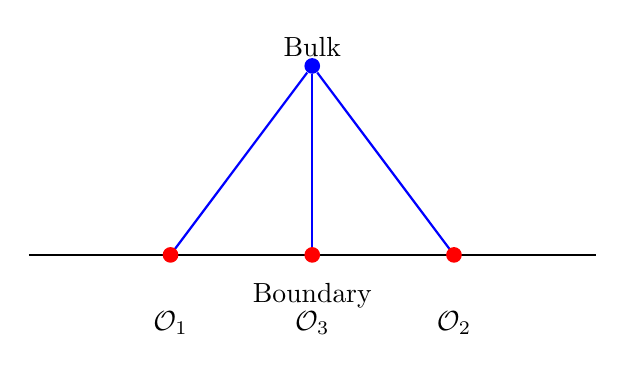
\begin{tikzpicture}[scale=1.2]
% Bulk point
\node[circle,fill=blue,inner sep=2pt] (bulk) at (0,2) {};
\node[above] at (bulk) {Bulk};

% Boundary line
\draw[thick] (-3,0) -- (3,0);
\node[below] at (0,-0.2) {Boundary};

% Propagators
\draw[blue,thick] (bulk) -- (-1.5,0);
\draw[blue,thick] (bulk) -- (1.5,0);
\draw[blue,thick] (bulk) -- (0,0);

% Boundary operators
\node[circle,fill=red,inner sep=2pt] at (-1.5,0) {};
\node[circle,fill=red,inner sep=2pt] at (1.5,0) {};
\node[circle,fill=red,inner sep=2pt] at (0,0) {};

\node[below] at (-1.5,-0.5) {$\mathcal{O}_1$};
\node[below] at (1.5,-0.5) {$\mathcal{O}_2$};
\node[below] at (0,-0.5) {$\mathcal{O}_3$};
\end{tikzpicture}
\end{center}

The OPE coefficient is:
$$C_{12}^3 = \int_{\text{bulk}} \langle \mathcal{O}_1 \mathcal{O}_2 \mathcal{O}_3^! \rangle_{\text{Witten diagram}}$$
where $\mathcal{O}_3^!$ is the Koszul dual operator.
\end{technique}

\begin{algorithm}[Computing Koszul Dual OPEs]\label{alg:koszul-ope}
\begin{algorithmic}
\STATE \textbf{Input:} Chiral algebra $\mathcal{A}$, operators $\mathcal{O}_1, \mathcal{O}_2$
\STATE \textbf{Output:} OPE in Koszul dual $\mathcal{A}^!$

\STATE \textbf{Step 1:} Compute bar complex elements
\STATE $\bar{\mathcal{O}}_i \gets \bar{B}(\mathcal{O}_i) \in \bar{B}(\mathcal{A})$

\STATE \textbf{Step 2:} Apply cobar construction
\STATE $\mathcal{O}_i^! \gets \Omega(\bar{\mathcal{O}}_i) \in \mathcal{A}^!$

\STATE \textbf{Step 3:} Compute pairing
\STATE $\langle \mathcal{O}_1^! \mathcal{O}_2^! \rangle \gets \text{Res}_{D_{12}}[\mu_{12} \otimes \eta_{12}]$

\STATE \textbf{Step 4:} Extract OPE
\STATE $\mathcal{O}_1^!(z) \mathcal{O}_2^!(w) \sim \sum_n \frac{C_n}{(z-w)^n}$
\STATE where $C_n$ from residue calculation

\RETURN OPE coefficients $\{C_n\}$
\end{algorithmic}
\end{algorithm}

\subsection{The AdS$_3$/CFT$_2$ Example: Twisted Supergravity}

\begin{example}[AdS$_3 \times S^3 \times T^4$ Holography]\label{ex:AdS3}
Following Costello-Paquette \cite{CP2020}, consider type IIB on AdS$_3 \times S^3 \times T^4$.

\textbf{Boundary:} The symmetric orbifold $\text{Sym}^N(T^4)$ as $N \to \infty$

\textbf{Bulk:} Twisted supergravity = Kodaira-Spencer theory

After twisting by a nilpotent supercharge $Q$ with $Q^2 = 0$:

\begin{center}
\begin{tabular}{|c|c|c|}
\hline
\textbf{Boundary} & $\leftrightarrow$ & \textbf{Bulk} \\
\hline
$Q$-cohomology of $\text{Sym}^N(T^4)$ & Koszul & Kodaira-Spencer on AdS$_3$ \\
Single-trace operators & duality & Gravitational modes \\
$W_{1+\infty}$ algebra & $\cong$ & Deformed $\text{Vir} \ltimes \text{Diff}(S^3)$ \\
\hline
\end{tabular}
\end{center}

The Koszul duality becomes:
$$\boxed{W_{1+\infty} \text{ at } c = 6N \quad \xleftrightarrow{\text{Koszul}} \quad \text{KS gravity on AdS}_3}$$
\end{example}

\begin{theorem}[Gravitational Backreaction and Deformation]\label{thm:backreaction}
The gravitational backreaction deforms the Koszul duality by:
\begin{enumerate}
\item Shifting generators by $\mathcal{O}(1/N)$ corrections
\item Modifying the differential: $d \to d + \delta d$ where $\delta d \sim g_s$
\item Curving the $A_\infty$ structure with $m_0 = \frac{1}{N}\text{Tr}(T^2)$
\end{enumerate}

The deformed pairing becomes:
$$\langle \mathcal{A}, \mathcal{B} \rangle_{\text{deformed}} = \langle \mathcal{A}, \mathcal{B} \rangle_0 + \sum_{n=1}^\infty \frac{1}{N^n} \langle \mathcal{A}, \mathcal{B} \rangle_n$$
where $\langle \cdot, \cdot \rangle_n$ includes $n$-loop gravitational corrections.
\end{theorem}

\subsection{Physical Interpretation: Defects and Open-Closed Duality}

\begin{interpretation}[Open-Closed String Duality]
The Koszul duality in holography realizes open-closed string duality:

\begin{center}
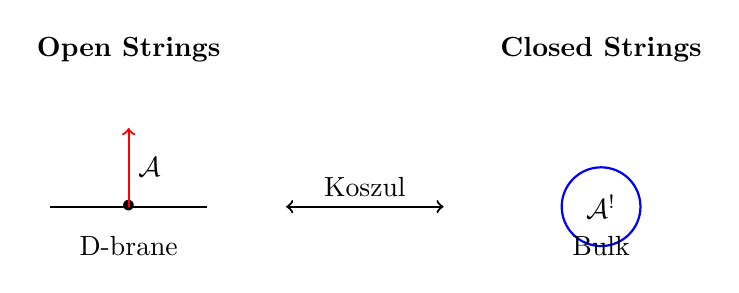
\begin{tikzpicture}[scale=1]
% Left side - Open strings
\node at (-3,2) {\textbf{Open Strings}};
\draw[thick] (-4,0) -- (-2,0);
\node at (-3,0) {$\bullet$};
\draw[red,thick,->] (-3,0) -- (-3,1);
\node[right] at (-3,0.5) {$\mathcal{A}$};
\node at (-3,-0.5) {D-brane};

% Arrow
\draw[<->,thick] (-1,0) -- (1,0);
\node[above] at (0,0) {Koszul};

% Right side - Closed strings
\node at (3,2) {\textbf{Closed Strings}};
\draw[blue,thick] (3,0) circle (0.5);
\node at (3,0) {$\mathcal{A}^!$};
\node at (3,-0.5) {Bulk};
\end{tikzpicture}
\end{center}

\begin{itemize}
\item Open string field theory on branes $\to$ Chiral algebra $\mathcal{A}$
\item Closed string field theory in bulk $\to$ Koszul dual $\mathcal{A}^!$
\item Disk amplitude with boundary $\mathcal{A}$ $=$ Sphere amplitude in $\mathcal{A}^!$
\end{itemize}
\end{interpretation}

\begin{theorem}[Universal Defect Construction]\label{thm:universal-defect-construction}
For any chiral algebra $\mathcal{A}$, the universal defect $\mathcal{D}(\mathcal{A})$ is constructed as:

$$\mathcal{D}(\mathcal{A}) = \bigoplus_{n=0}^\infty \text{Ext}^n_{\mathcal{A}}(\mathbb{C}, \mathbb{C})$$

with multiplication given by Yoneda product. This satisfies:
\begin{enumerate}
\item \textbf{Functoriality:} $\mathcal{A} \to \mathcal{B}$ induces $\mathcal{D}(\mathcal{B}) \to \mathcal{D}(\mathcal{A})$
\item \textbf{Universality:} Any defect factors through $\mathcal{D}(\mathcal{A})$
\item \textbf{Duality:} $\mathcal{D}(\mathcal{D}(\mathcal{A})) \simeq \mathcal{A}$ (under mild conditions)
\end{enumerate}
\end{theorem}

\subsection{Complete Examples and Computations}

\subsubsection{Example: Free Fermion and its Koszul Dual}

\begin{example}[Free Fermion $\leftrightarrow$ $\beta\gamma$ System]
The free fermion $\psi$ with OPE $\psi(z)\psi(w) \sim (z-w)^{-1}$ is Koszul dual to the $\beta\gamma$ system:

$$\boxed{\text{Free fermion } \psi \quad \xleftrightarrow{\text{Koszul}} \quad \beta\gamma \text{ system}}$$

\textbf{Bar complex of fermion:}
\begin{align}
\bar{B}^0(\psi) &= \mathbb{C} \\
\bar{B}^1(\psi) &= \text{span}\{\psi_1 \otimes \psi_2 \otimes \eta_{12}\} \\
\bar{B}^2(\psi) &= 0 \text{ (fermionic constraint)}
\end{align}

\textbf{Cobar gives $\beta\gamma$:}
\begin{align}
\Omega^0 &= \mathbb{C} \\
\Omega^1 &= \text{span}\{\beta, \gamma\} \\
\beta(z)\gamma(w) &\sim \frac{1}{z-w}
\end{align}

The pairing:
$$\langle \psi \otimes \psi, \beta \otimes \gamma - \gamma \otimes \beta \rangle = 1$$
encodes the Koszul duality.
\end{example}

\subsubsection{Example: Heisenberg and W-algebras}

\begin{example}[Heisenberg $\leftrightarrow$ W-algebra]
The Heisenberg algebra at level $k$ is related to W-algebras by curved Koszul duality:

$$\mathcal{H}_k \xleftrightarrow{\text{curved Koszul}} W^{-k-h^\vee}(\mathfrak{g})$$

where $h^\vee$ is the dual Coxeter number.

The curvature:
$$m_0 = \frac{k + h^\vee}{12} \cdot c_{\text{Sugawara}}$$
measures the failure of strict duality.
\end{example}

\subsubsection{Complete Calculation: Yangian from M2 Branes}

\begin{calculation}[Yangian Structure Constants]
For M2 branes, the Yangian generators $\{E_{ij}^{(r)}\}$ satisfy:

$$[E_{ij}^{(r)}, E_{k\ell}^{(s)}] = \delta_{jk}E_{i\ell}^{(r+s)} - \delta_{i\ell}E_{kj}^{(r+s)} + \hbar \sum_{t=1}^{\min(r,s)-1} \left(E_{i\ell}^{(t)}E_{kj}^{(r+s-t)} - E_{kj}^{(t)}E_{i\ell}^{(r+s-t)}\right)$$

These are computed from the Koszul dual via:
\begin{enumerate}
\item Take generators of $U(\text{Diff}(\mathbb{C}) \otimes \mathfrak{gl}_N)$
\item Compute bar complex (configuration space integrals)
\item Apply cobar construction
\item Extract structure constants from residues
\end{enumerate}

Explicit first few:
\begin{align}
[E_{ij}^{(0)}, E_{jk}^{(0)}] &= E_{ik}^{(0)} \\
[E_{ij}^{(0)}, E_{jk}^{(1)}] &= E_{ik}^{(1)} \\
[E_{ij}^{(1)}, E_{jk}^{(1)}] &= E_{ik}^{(2)} + \hbar(E_{ik}^{(0)})^2
\end{align}
\end{calculation}

\subsection{Applications and Future Directions}

\begin{applications}
\textbf{1. Holographic Correlators:}
$$\langle \mathcal{O}_1 \cdots \mathcal{O}_n \rangle_{\text{CFT}} = \int_{\text{AdS}} \mathcal{O}_1^! \cdots \mathcal{O}_n^! \cdot e^{-S_{\text{gravity}}}$$

\textbf{2. Quantum Groups from Gravity:}
Every AdS gravity theory yields a quantum group via Koszul duality

\textbf{3. Categorification:}
$$\text{D}^b(\mathcal{A}\text{-mod}) \simeq \text{D}^b(\mathcal{A}^!\text{-mod})^{\text{op}}$$

\textbf{4. Higher Spin Gravity:}
Vasiliev theory = Koszul dual of higher spin algebra
\end{applications}
